\section{Numerical validations for error estimations in energy}\label{sec:numeric_energy}

In this section, we present supplementary results for the numerical validations for error estimations in electrostatic energy, complementing the main text. Figures~\ref{fig:icm_error} to~\ref{fig:error_icm_pad_gamma_1} correspond one-to-one with Figures 1 to 4 in the main text, maintaining the same systems and parameter settings as those used in the force calculation results. The dashed lines in these figures represent the fitted curves based on our theoretical estimation given in Eq.~(52) of the main text. The energy error results exhibit similar trends to the force errors and align well with our theoretical predictions.


\begin{figure}[htbp]
    \centering
    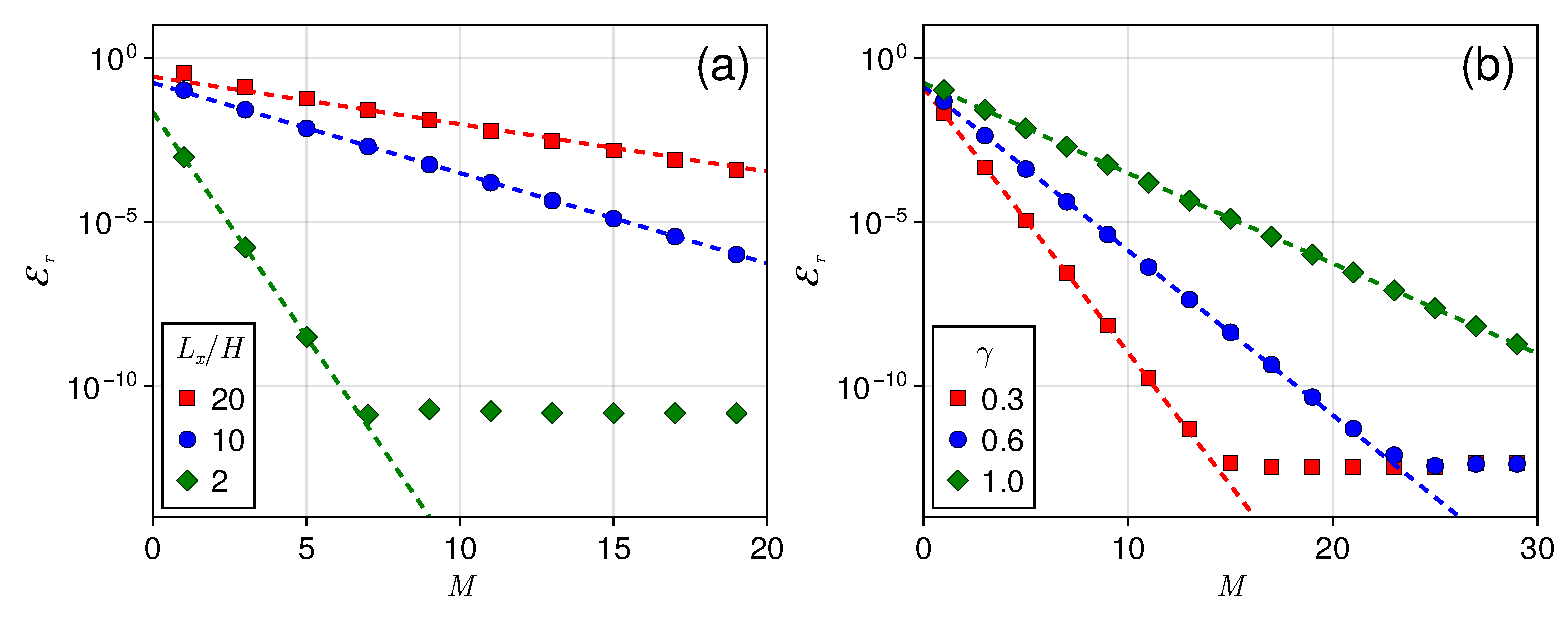
\includegraphics[width=0.98\linewidth]{figs/icm_error.pdf}
    \caption{
        Relative errors of energy due to truncation of image charges are presented. The dashed lines represent the fitted decay rate, as described in Eq. (54) in the main text. In panel (a) we set $\gamma_{\T u} = \gamma_{\T d} = 1$ and consider system heights of $H = 0.5, 1$ and $5$. In panel (b), we set $H = 1$ while varying $\gamma_{\T u} = \gamma_{\T d} = \gamma = 0.3, 0.6$ and $1$. 
        %The scope of the fitted lines are fixed to be $\lg(\gamma e^{-2\pi H / L_x})$, which is the theoretical value.
    }
    \label{fig:icm_error}
\end{figure}


\begin{figure}[htbp]
    \centering
    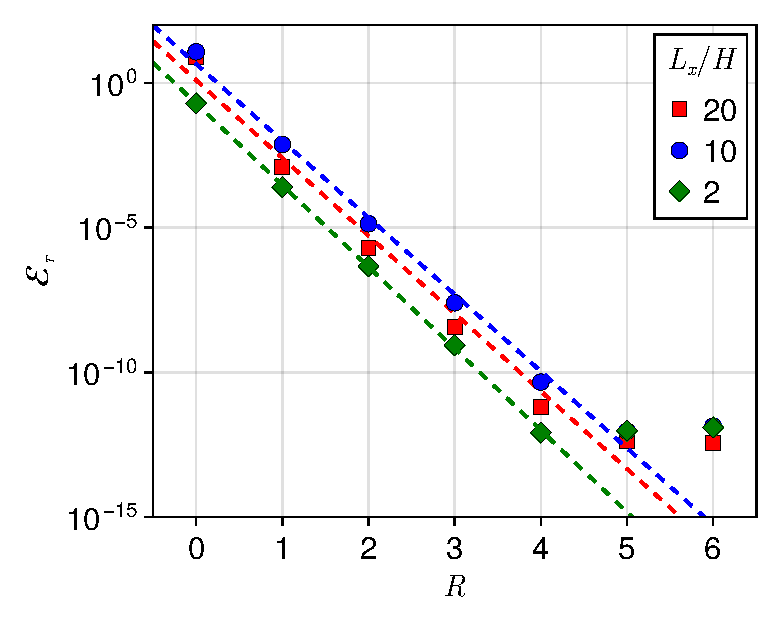
\includegraphics[width=0.49\linewidth]{figs/elc_error.pdf}
    \caption{Relative error of energy of reformulating the Ewald2D summation as 3D ones are presented. We set $\gamma_{\T u} = \gamma_{\T d} = 0$ and consider system heights of $H = 0.5, 1, 5$. Here $P = (L_z - H) / L_x$ denotes the padding ratio.}
    \label{fig:elc_error}
\end{figure}

\begin{figure}[htbp]
    \centering
    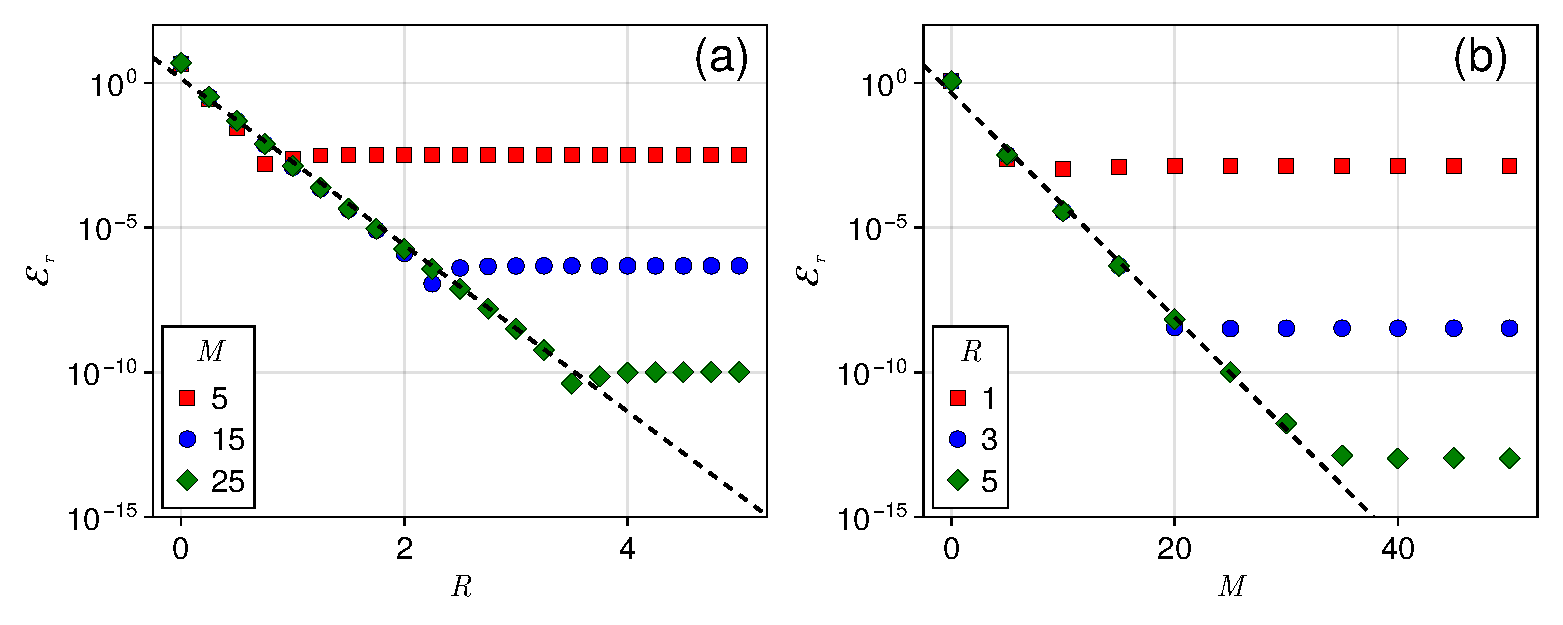
\includegraphics[width=0.98\linewidth]{figs/error_icm_pad_gamma_0.6.pdf}
    \caption{Relative error of energy in dielectric-confined Coulomb system with parameters $\gamma_{\T u} = \gamma_{\T d} = \gamma = 0.6$ and $H = 0.5$. Panel (a) illustrates error evolution with fixed image charge layers ($M = 5,~15,~25$) under varying padding ratios ($P$), whereas panel (b) demonstrates error progression with fixed $P = 1,~3,~5$ across increasing $M$.}
    \label{fig:error_icm_pad_gamma_0.6}
\end{figure}

\begin{figure}[htbp]
    \centering
    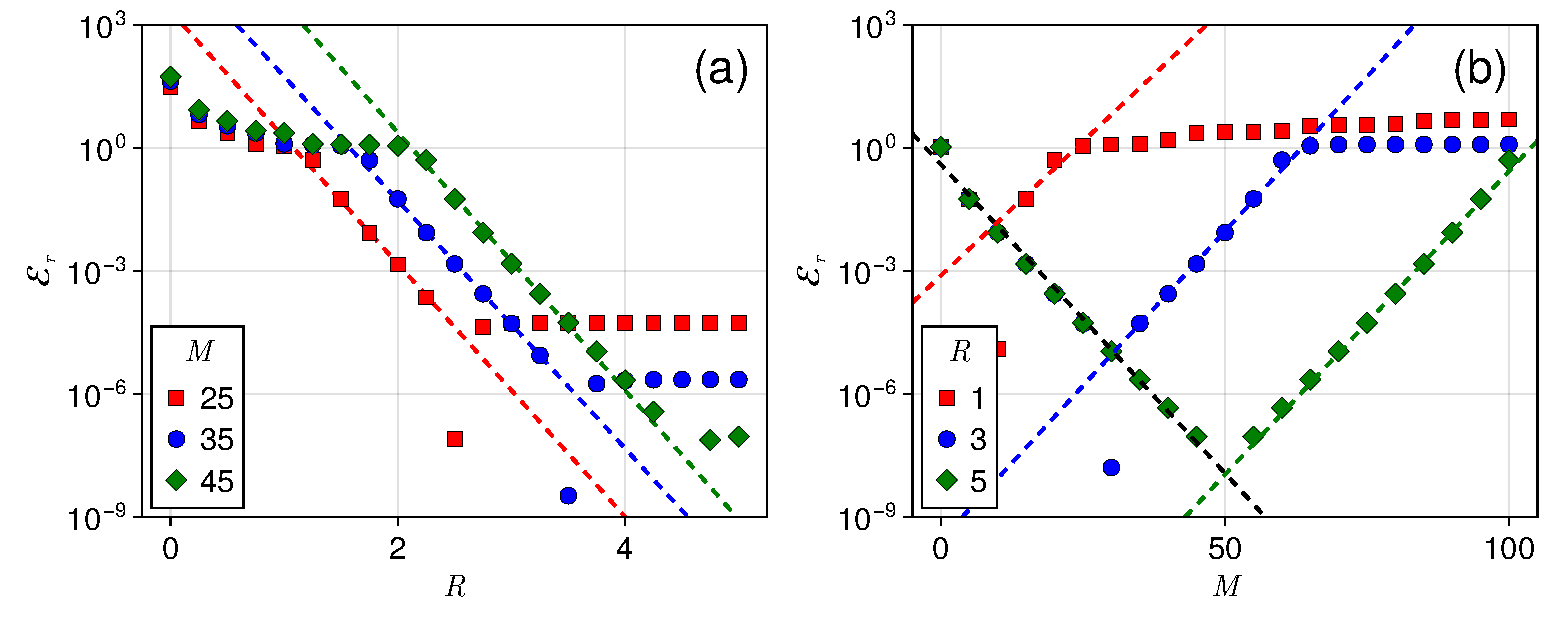
\includegraphics[width=0.98\linewidth]{figs/error_icm_pad_gamma_1.pdf}
    \caption{Relative error of energy in dielectric-confined Coulomb system with parameters $\gamma_{\T u} = \gamma_{\T d} = \gamma = 1$ and $H = 0.5$. Panel (a) illustrates error evolution with fixed image charge layers ($M = 5,~15,~25$) under varying padding ratios ($P$), whereas panel (b) demonstrates error progression with fixed $P = 1,~3,~5$ across increasing $M$.}
    \label{fig:error_icm_pad_gamma_1}
\end{figure}

\section{Challenge associated with strongly-confined systems}
In practical simulations, such as when studying thin membranes, ion transport in slit channels and supercapacitors, accurately capturing the effects of nanoconfinement, i.e., when $L_{x,y} / H\gg 1$, is crucial.
Previous numerical studies have found that more image layers are needed to achieve satisfactory accuracy for confined systems~\cite{dos2015electrolytes}. 
To further investigate the numerical properties of strongly-confined systems, we present the errors in force in Fig.~\ref{fig:icm_elc_error_force}, where we fix $L_x=L_y=10$, $P=(L_z-H)/L_x = 5$ and consider system heights $H = 0.5, 1, 5$ while varying the number of image charge layers $M$. 
In Fig.~\ref{fig:icm_elc_error_force} (a), for $\gamma = 0.6$, we observe that the error decays exponentially as $M$ increases for $H = 0.5$ and $H = 1$. 
However, for $H = 5$, where $|g_{\T u}g_{\T d}|>1$, the error becomes non-monotonic as $M$ increases, 
which is consistent with our theoretical predictions as discussed in the main text.
In Fig.~\ref{fig:icm_elc_error_force} (b), with $\gamma = 1$, we observe a similar non-monotonic pattern for all aspect ratios. 
It is important to note that, the rate of error decrease/increase depends on the aspect ratio $L_x/H$. 
A higher aspect ratio leads to a slower increase or decrease in errors, as $M$ is less or greater than the critical value that minimizes the error, respectively. 
This also highlights the computational challenge associated with strongly-confined systems -- to achieve the same accuracy, a much larger $M$ is required compared to non-confined systems.
Same conclusions hold for the errors in energy, as shown in Fig.~\ref{fig:icm_elc_error}.

\begin{figure}[htbp]
    \centering
    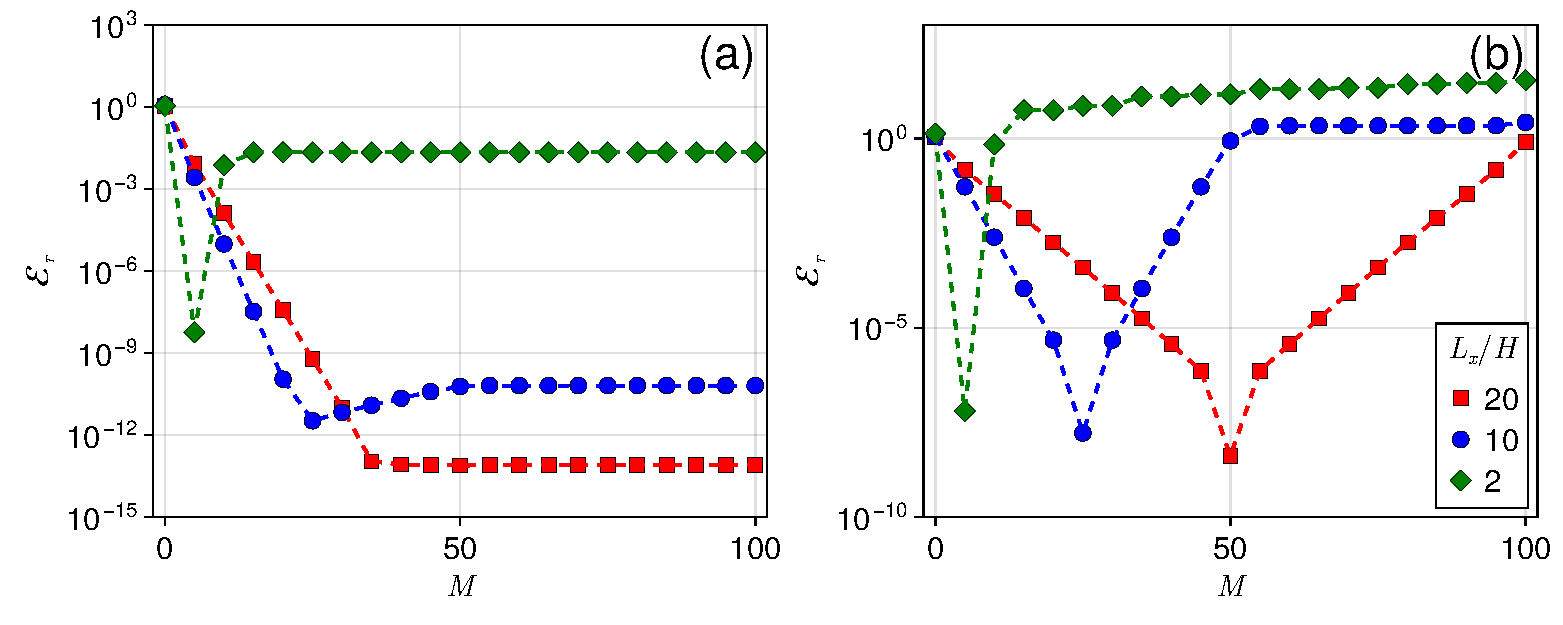
\includegraphics[width=0.98\linewidth]{figs/icm_elc_error_force.pdf}
    \caption{Relative error of force ($\mathcal{E}_r$) in a dielectric-confined Coulomb system with parameters $P = 5$ and $H = 0.5, 1, 5$. In panels (a) and (b), the dielectric contrasts are set to $\gamma_{\T u} = \gamma_{\T d} = \gamma = 0.6$ and $\gamma_{\T u} = \gamma_{\T d} = \gamma = 1$, respectively.}
    \label{fig:icm_elc_error_force}
\end{figure}

\begin{figure}[htbp]
    \centering
    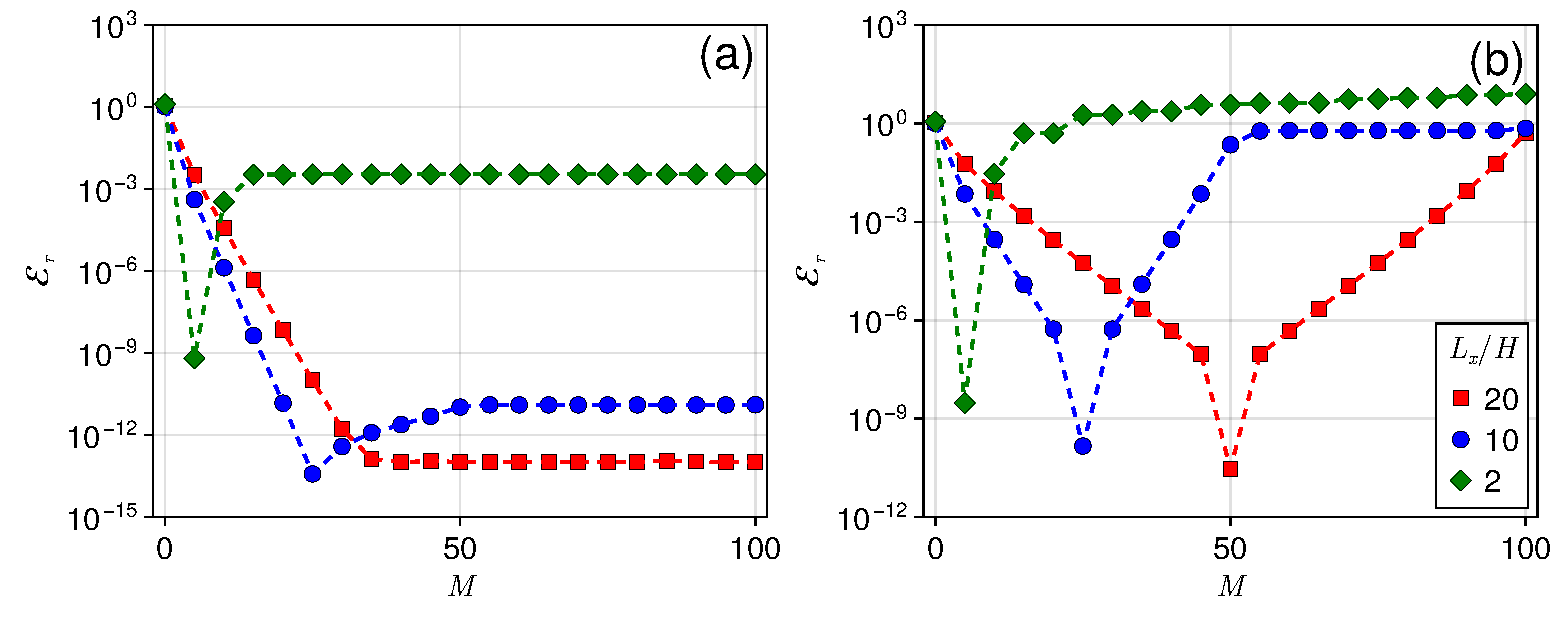
\includegraphics[width=0.98\linewidth]{figs/icm_elc_error.pdf}
    \caption{Relative error of energy in a dielectric-confined Coulomb system with parameters $P = 5$ and $H = 0.5, 1, 5$. In panels (a) and (b), the dielectric contrasts are set to $\gamma_{\T u} = \gamma_{\T d} = \gamma = 0.6$ and $\gamma_{\T u} = \gamma_{\T d} = \gamma = 1$, respectively.}
    \label{fig:icm_elc_error}
\end{figure}

\section{Quadrature error of the trapezoidal rule}\label{app::trapezoidal}
We employ the method of contour integrals~\cite{Donaldson1972SINUA,trefethen2014Rev} to derive a precise estimation for the error in  {the} trapezoidal rule when discretizing Eqs.~\eqref{eq:ewald2d-intform1} and \eqref{eq::J02}. Consider the integral
\begin{equation}\label{eq::A.1}
I=\int_{-\infty}^{\infty }\frac{e^{-(a^2+t^2)}}{a^2+t^2}e^{\i b t}dt,
\end{equation}
where $a\geq 0$ and $b\in\mathbb{R}$. We approximate $I$ using a $(2M+1)$-point trapezoidal rule:
\begin{equation}
I_{M,\xi}=\xi\sum_{j=-M}^{M}\frac{e^{-a^2-(j\xi)^2}}{a^2+(j\xi)^2}e^{\i b j\xi},
\end{equation}
where $\xi>0$ is the step size, and we define the remainder as $E_{M,\xi}:=I-I_{M,\xi}$. Note that the integrand of $I$ has two simple poles at $t_{\pm}=\pm \i a$. Let $\Gamma_{\pm}$ be two positively/negatively oriented rectangular contours with vertices $(M+1/2)\xi\pm\i a^*$, $-(M+1/2)\xi\pm\i a^*$, $(M+1/2)\xi$, and $-(M+1/2)\xi$ (see Fig.~\ref{fig:Trapezoidal}). We enforce $a^*>a$ so that $\Gamma_{\pm}$ encloses both the interval $[-M \xi,M \xi]$ and the pole $t_{\pm}$. By following the approach given in~\cite{Donaldson1972SINUA} and applying Cauchy's theorem, we can derive an estimate for $E_{M,\xi}$ in the limit $M\rightarrow \infty$:
\begin{equation}
E_{M,\xi}=\int_{\Gamma_++\Gamma_-}\frac{e^{-(a^2+t^2)+\i b t}}{a^2+t^2}\varphi(t)dt-2\pi\i \text{Res}\left[\frac{e^{-(a^2+t^2)+\i b t}}{a^2+t^2}\varphi(t),\pm \i a\right],
\end{equation}
where
\begin{align}
\varphi(t)=\begin{cases}
\dfrac{1}{1-e^{2\pi\i t/\xi}},\,\quad &\text{Im}(t)<0,\\[1em]
-\dfrac{1}{1-e^{-2\pi\i t/\xi}},\,\quad&\text{Im}(t)>0,
\end{cases}
\end{align}
is related to the characteristic function of the trapezoidal rule, and $\text{Res}[f(t),t_0]$ denotes the residue of a function $f$ at a pole $t_0$. Since the contributions from the vertical sides of $\Gamma_{\pm}$ vanish in the limit $M\rightarrow \infty$ and by using residue calculus, we have
\begin{equation}\label{eq::A.5}
E_{M,\xi}=\left(\int_{-\infty+\i a^*}^{\infty+\i a^*}-\int_{-\infty-\i a^*}^{\infty-\i a^*}\right)\frac{e^{-(a^2+t^2)+\i b t}}{a^2+t^2}\varphi(t)dt+\frac{\pi}{a}\frac{e^{-ab}+e^{ab}}{1-e^{2\pi a/\xi}}.
\end{equation}
In Eq.~\eqref{eq::A.5}, the last term can be considered as the residue correction of the rule, while the remainder integral along $\text{Im}(t)=a^*$ can be estimated as
\begin{equation}
\begin{split}
\left|\int_{-\infty+\i a^*}^{\infty+\i a^*}\frac{e^{-(a^2+t^2)+\i b t}}{a^2+t^2}\varphi(t)dt\right|&\leq e^{(a^*)^2-a^2-a^*b-2\pi a^*/\xi}\int_{-\infty}^{\infty}\frac{|a^2+(t+\i a^*)^2|^{-1}e^{-t^2}}{\left|1-e^{2\pi\i t/\xi-2\pi a^*/\xi}\right|}dt\\
&\leq\frac{\sqrt{\pi}e^{(a^*)^2-a^2-a^*b-2\pi a^*/\xi}}{(a^*)^2-a^2}.
\end{split}
\end{equation}

To obtain a closed formula, it is necessary to determine the extremum of the exponent under the condition $a^*>a>0$. Since the range of $a$ is not specified, we can safely choose $a^*=\pi/\xi+b/2$ if $\pi/\xi+b/2>a$, and $a^*=\sqrt{a^2+1}$ otherwise. This choice ensures a decay rate of at least $\sim\mathcal{O}(e^{-\text{sign}(\pi/\xi+b/2)|\pi/\xi+b/2|^2})$, where $\text{sign}(t)=1$ if $t> 0$, $\text{sign}(t)=0$ if $t=0$, and $\text{sign}(t)=-1$ otherwise. By following a similar procedure, we can derive that the integral along $\text{Im}(t)=-a^*$ in Eq.~\eqref{eq::A.5} decays with order $\mathcal{O}(e^{-\text{sign}(\pi/\xi-b/2)|\pi/\xi-b/2|^2})$. Consequently, we can conclude that
\begin{equation}
E_{M,\xi}=\frac{\pi}{a}\frac{e^{-ab}+e^{ab}}{1-e^{2\pi a/\xi}}+E_{\text{err}},
\end{equation}
where the remainder error term can be estimated as 
\begin{equation}\label{eq::A.8}
|E_{\text{err}}|\sim \mathcal{O}(e^{-\text{sign}(\pi/\xi-|b|/2)\left|\pi/\xi-|b|/2\right|^2}).
\end{equation}

\begin{figure}[!ht]
    \begin{center}
    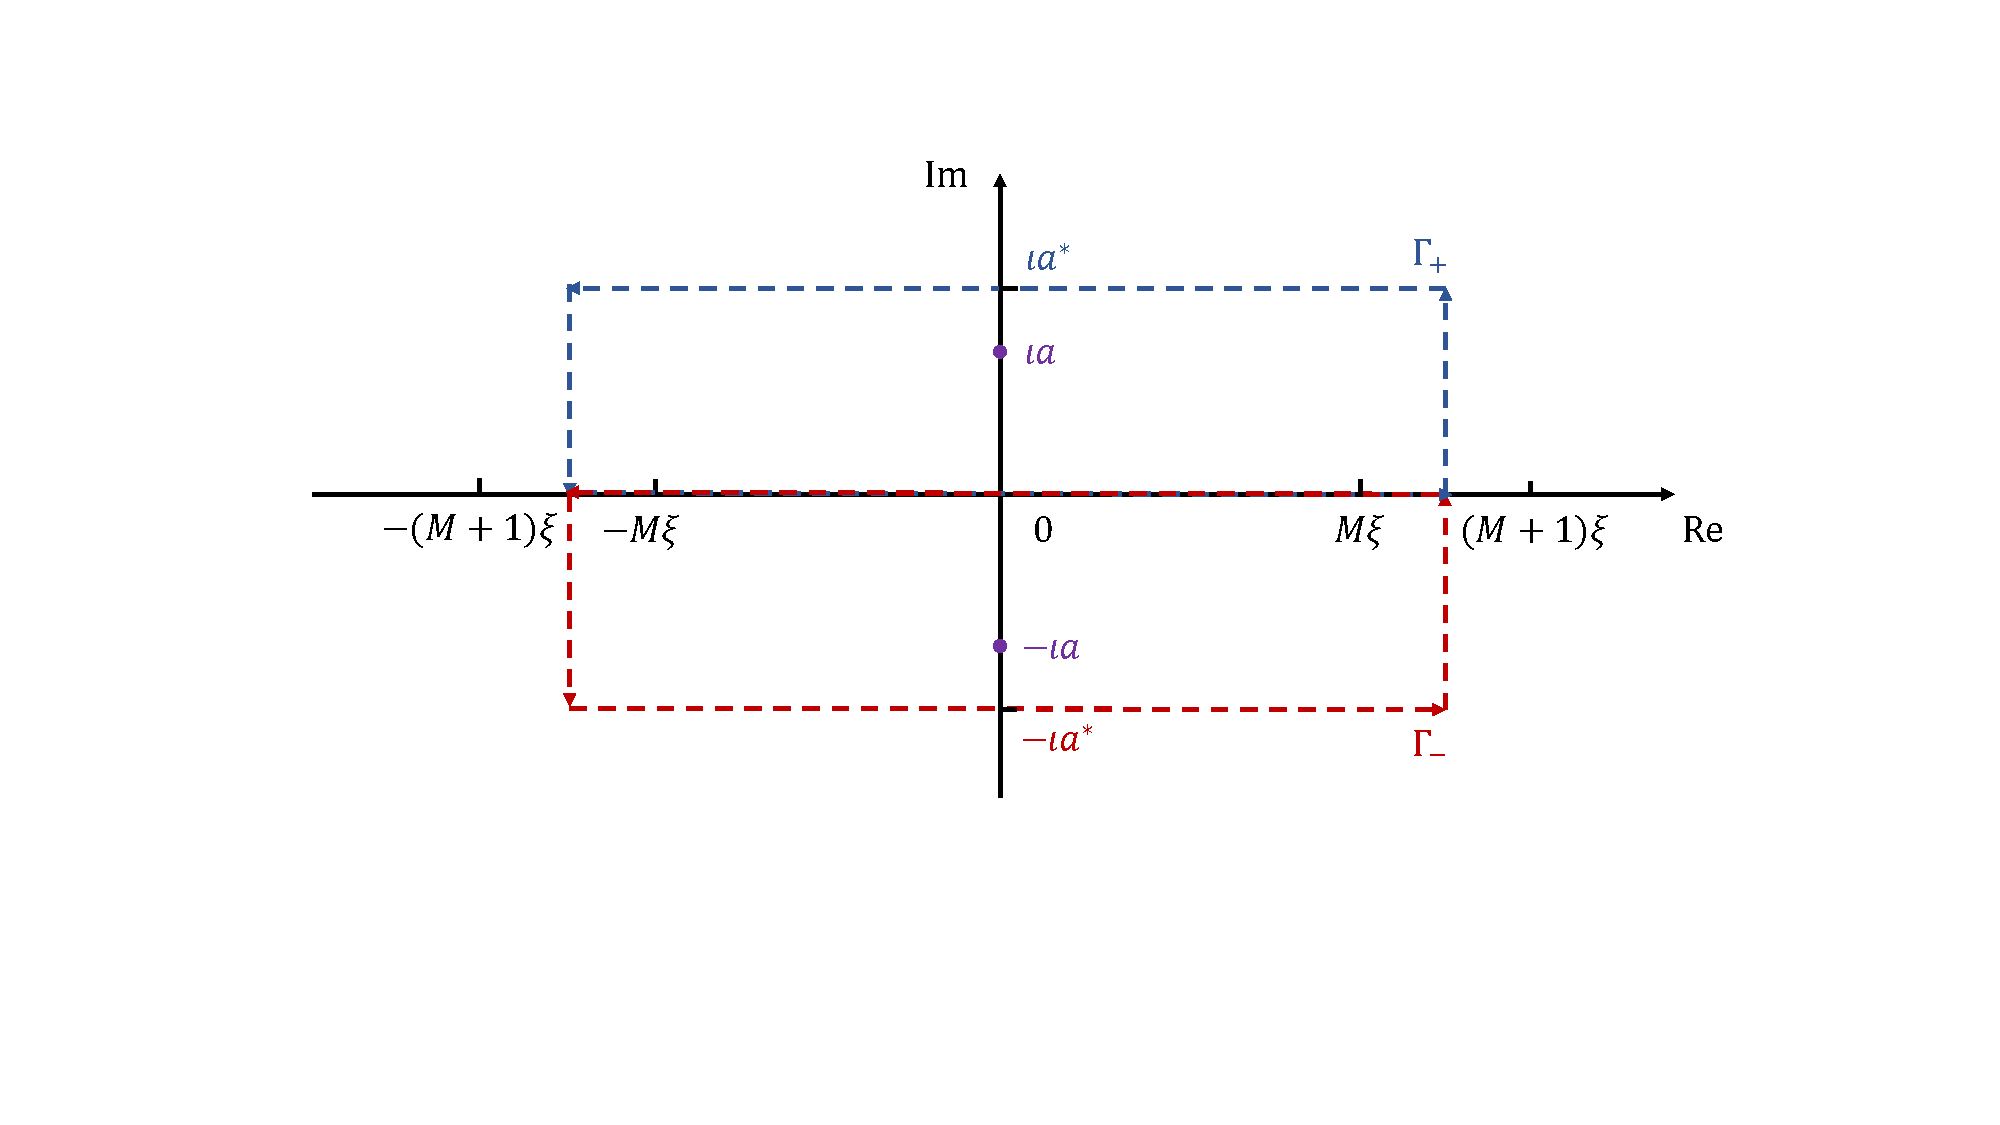
\includegraphics[width=0.8\textwidth]{figs/Trapezoidal.pdf}
    \caption{Integration contours in the error estimation of trapezoidal rule.}
    \label{fig:Trapezoidal}
    \end{center} 
\end{figure}

\section{Quasi-2D systems with charged slab walls}\label{app::surfacecharge}

In this section, we will discuss the extension of the developed RBE algorithm to handle systems that involve both continuous surface charges and free ions. Without loss of generality, we assume two charged interfaces are located at $z=0$ and $z=H$ and with uniform surface charge density $\sigma_{\text{bot}}$ and $\sigma_{\text{top}}$. The system satisfies the charge neutrality condition \begin{equation}\label{eq::chargeneutrality}
    \sum_{i=1}^N q_i+(\sigma_{\text{bot}}+\sigma_{\text{top}})L_xL_y=0\;,
\end{equation}
so that the electrostatic energy and force of the system are both well-defined. When dealing with surface charges, it is common in the literature to handle discrete ions and continuous surface charges separately~\cite{spohr1997effect,yi2017note,yuan2021particle}. The former is typically treated as an infinite summation problem, while the latter is often obtained by solving an additional Poisson equation. %However, during the energy calculation, some divergent terms may arise. Since these terms do not affect the forces, they are often disregarded in a rough manner. 

In this manuscript, we employ a unified methodology where the continuous charge is treated as the limit distribution of an infinite set of discrete charges, following the framework outlined in Theorem~\ref{thm::FourDie}. To ensure accuracy, the parameters $M$ and $L_z$ are carefully selected to render both the ELC and remainder error terms negligible. As a result, we can accurately describe the force exerted on each mobile ion as:
\begin{equation}
\bm{F}^{\text{c}}(\bm{r}_i)=\bm{F}^{\text{c}}_{\text{real}}(\bm{r}_i)+\bm{F}^{\text{c}}_{\text{Fourier}}(\bm{r}_i)+\bm{F}^{\text{c}}_{\text{wall}}(\bm{r}_i),
\end{equation}
including the real space, the Fourier space, and ion-wall components. The real space component is given by
\begin{equation}\label{eq::F_real_detail}
\begin{split}
\bm{F}_{\text{real}}^{\te{c}}(\bm{r}_i)
& := -q_i\sum_{j=1}^{N} q_j \Biggg[\sum_{\bm{n}}{}^\prime \frac{\left(\bm{r}_{i,\bm{n}} - \bm{r}_{j}\right)}{\abs{\bm{r}_{i,\bm{n}} - \bm{r}_{j}}} K(\abs{\bm{r}_{i,\bm{n}} - \bm{r}_{j}}) + \frac{1}{2} \sum_{\bm{n}} \sum_{l=1}^{M} \frac{\gamma_{l}^+\left(\bm{r}_{i,\bm{n}}-\bm{r}_{j+}^{(l)}\right)}{\left|\bm{r}_{i,\bm{n}}-\bm{r}_{j+}^{(l)}\right|} K\left(\left|\bm{r}_{i,\bm{n}}-\bm{r}_{j+}^{(l)}\right|\right)\\
+&\frac{1}{2}\sum_{\bm{n}}\sum_{l=1}^{M}\frac{\gamma_{l}^-\left(\bm{r}_{i,\bm{n}}-\bm{r}_{j-}^{(l)}\right)}{\left|\bm{r}_{i,\bm{n}}-\bm{r}_{j-}^{(l)}\right|}K\left(\left|\bm{r}_{i,\bm{n}}-\bm{r}_{j-}^{(l)}\right|\right)\Biggg]-\frac{q_i}{2}\sum_{j=1}^{N}q_j\sum_{\bm{n}}\sum_{l=1}^{M}\begin{pmatrix}
1&0&0\\
0&1&0\\
0&0&(-1)^l
\end{pmatrix}\\\Biggg[&
\frac{\gamma_{l}^+\left(\bm{r}_{i,\bm{n}}-\bm{r}_{j+}^{(l)}\right)}{\left|\bm{r}_{i,\bm{n}}-\bm{r}_{j+}^{(l)}\right|}K\left(\left|\bm{r}_{i,\bm{n}}-\bm{r}_{j+}^{(l)}\right|\right)+\frac{\gamma_{l}^-\left(\bm{r}_{i,\bm{n}}-\bm{r}_{j-}^{(l)}\right)}{\left|\bm{r}_{i,\bm{n}}-\bm{r}_{j-}^{(l)}\right|}K\left(\left|\bm{r}_{i,\bm{n}}-\bm{r}_{j-}^{(l)}\right|\right)\Biggg]
\end{split}
\end{equation}
where $\bm{r}_{i,\bm{n}}=\bm{r}_{i}+\bm{\ell}$, and $K(r):=\text{erfc}(\alpha r)/r^2+2\alpha e^{-\alpha^2r^2}/(\sqrt{\pi}r)$. The Fourier component of force, $\bm{F}^{\text{c}}_{\text{Fourier}}$, has been provided in Eq.~\eqref{eq::52}. In practice, we use the RBE force $\bm{F}^{\text{c},*}_{\text{Fourier}}$ in Eq.~\eqref{eq::important} as an unbiased estimator to $\bm{F}^{\text{c}}_{\text{Fourier}}$, in which the formula of IBC term is more complicated than  {in} the case of  {a} neutral interface:
\begin{equation}\label{eq::IBC}
\begin{split}
\bm{F}_{\text{IBC}}^{M}(\bm{r}_i)=&-\frac{2\pi q_{i}}{L_xL_yL_z}\left[\mathcal{M}_{z}\left(1+\sum_{l=1}^{M}(-1)^{l}\left(\gamma_{+}^{(l)}+\gamma_{-}^{(l)}\right)\right)+\mathcal{M}_{z}^{M}\right]\V{\hat e_z}\\
&+\frac{2\pi q_i}{L_xL_yL_z}\sum_{j=1}^{N}q_j\left[z_i+\sum_{l=1}^{M}(-1)^{l}\left(\gamma_{+}^{(l)}z_{i+}^{(l)}+\gamma_{-}^{(l)}z_{i-}^{(l)}\right)\right]\V{\hat e_z}\\
&+\frac{2\pi q_iz_i}{L_xL_yL_z}\sum_{j=1}^{N}q_j\left[1+\sum_{l=1}^{M}\left(\gamma_{+}^{(l)}+\gamma_{-}^{(l)}\right)\right]\V{\hat e_z},
\end{split}
\end{equation}
where the $z$-direction dipole moments are defined via
\begin{equation}
\mathcal{M}_{z}:=\sum_{i=1}^{N}q_iz_i\quad\text{and}\quad \mathcal{M}_{z}^{M}:=\sum_{i=1}^{N}q_i\left[z_{j}+\sum_{l=1}^{M}\left(\gamma_{+}^{(l)}z_{j+}^{(l)}+\gamma_{-}^{(l)}z_{j-}^{(l)}\right)\right].
\end{equation}
It is important to highlight that if the free ions in the solution continue to fulfill condition Eq.~\eqref{eq:neutrality}, the last two terms in Eq.~\eqref{eq::IBC} vanish. 
The ion-wall component represents the force exerts on the mobile ions due to the charged walls, and is given by
\begin{equation}
\bm{F}_{\text{wall}}^{\te{c}}:=-2\pi z_{i}q_{i}\left[\sigma_{\text{top}}-\sigma_{\text{bot}}+\frac{(\sigma_{\text{top}}+\sigma_{\text{bot}})(\gamma_{\text{top}}-\gamma_{\text{bot}})\left(1-\gamma_{\text{top}}^{\lceil M/2 \rceil}\gamma_{\text{bot}}^{\lceil M/2 \rceil}\right)}{1-\gamma_{\text{top}}\gamma_{\text{bot}}}\right]\V{\hat e_z}.
\end{equation}

\section{Physical quantities evaluated in results}\label{Sec::phyquan}

In this section, we will briefly describe how to calculate the physical quantities of interest in this paper.

To calculate the average concentration of the system along the $z$-direction, we first divide the interval $[0,H]$ into $250$ equally spaced bins. Then, every $100$ steps, we count the number of particles whose $z$-coordinate $r_z$ falls within each bin and calculate the ensemble average. After the simulation is completed, we divide the accumulated values by the length of each bin to obtain the average concentration. The MSD along $z$-direction, $\eta_{\text{msd},z}(t)$ at time $t$ is defined as
\begin{equation}
\eta_{\mathrm{msd},z}(t)=\left\langle\left|r_z\left(t+t_0\right)-r_z\left(t_0\right)\right|^2\right\rangle,
\end{equation}
with the bracket representing the ensemble average over $t_0$. The VACF along $z$-direction, $\eta_{\text{vacf},z}(t)$ at time $t$ is defined as
\begin{equation}
\eta_{\text {vacf},z}(t)=\left\langle v_z\left(t_0\right) v_z(t)\right\rangle,
\end{equation}
with the bracket representing the ensemble average over $t_0$. The total energy is defined as the sum of potential energy and kinetic energy. The potential energy is the sum of bond, angle, Coulomb, LJ and  {constraint} components, where the first two and the last one are not required for electrolyte solutions. 

Let $N$ is the number of particles, $\bm{r}_i=(r_{i,x},r_{i,y},r_{i,z})$, $\bm{v}_i=(v_{i,x},v_{i,y},v_{i,z})$ and $\bm{f}_i=(f_{i,x},f_{i,y},f_{i,z})$ represent the position, velocity and force of $i$th particle along each of three dimensions, respectively. The $z$-$z$ component subtracted from pressure tensor is computed by the formula
\begin{equation}
P_{zz}=\frac{1}{V} \sum_{i=1}^N\left(m_i v_{i,z} v_{i, z}+r_{i,z} f_{i,z}\right),
\end{equation}
where the two components in each term come from the kinetic energy and the virial contributions, respectively. It is remarked that the far-field component of  {the} virial associated with the Ewald decomposition requires the use of specialized methods~\cite{liang2022random}. 

% \section{High-performance implementation}\label{sec::ImpleStr}
% The RBE2D method is highly suitable for parallelization and vectorization. In this section, we present our implementation strategy for the RBE2D, incorporating MPI parallelization and Intel 512-bit SIMD (AVX-512 architecture) for vectorization. The latter enables simultaneous calculations of sixteen neighbors for single-precision floating-point operations (or eight for double precision). Intel One-API is employed for parallelization, encompassing MPI and AVX-512 instructions. The approach presented here is equally applicable to other parallelization models and vectorization instructions.

% Our implementation contributes in two main aspects. Firstly, we design communication operations that overlap with computations, reducing the overall serial portion. Secondly, we reformulate the expressions for the Fourier component and the dielectric correction component of the Coulomb interaction to reduce computational complexity. We discuss the techniques and insights as follows. Although these details may seem unrelated to the scientific aspects, we believe they are crucial for readers who are interested to reproduce or even improve upon our work.

% Due to the mini-batch strategy in the Fourier space, a serial importance sampling procedure and a global broadcast operation are required at each MD step. However, we mitigate this cost through the designed non-jammed communication, computation/communication overlapping, and parallel execution. Here are the details: assuming $\mathcal{M}$ MPI ranks are employed, $\mathcal{M}$ independent sampling processes are executed in parallel within each rank. The $1$st MPI rank broadcasts the samples to other ranks using a blocking operation. Concurrently, the computation step of the Coulomb interaction is executed while the samples in the $2$nd MPI rank are being broadcasted. This sequence is repeated $\mathcal{M}-1$ times, followed by a new sampling loop. This strategy evaluates and updates the samples every $\mathcal{M}$ steps, significantly reducing the sampling and global communication costs. It is crucial to emphasize that in order to generate independent samples, it is necessary for each rank to utilize a distinct initial random number seed.

% The image charge reflection, which accounts for dielectric jumps, is efficiently handled by precomputing the coefficients, as described in Section~\ref{sec::imagecharge}. This step, which incurs substantial computational resources in previous FFT-based methods~\cite{yuan2021particle}, involves lower additional costs in the RBE2D method developed in this paper.

% Furthermore, the speedup of the RBE2D is limited by the cost of the real-space calculation, specifically the computation of $F_i^{\text{real}}$. To enhance efficiency in the real space, the RBE2D implementation adopts the procedure from LAMMPS \cite{plimpton1995fast}, including domain decomposition, cell lists, communication design, and data structures. The directive-based offload technique \cite{brown2015optimizing} is employed for further acceleration. The computationally expensive error complementary function is efficiently computed using a combination of Taylor expansion, bit masking, and table look-up techniques, following the approach of LAMMPS.

% In many works that employ FFT-based methods as their electrostatic solvers, the real-space cutoff is balanced to ensure that the costs of the real and Fourier spaces are approximately equal. For the RBE2D, the real-space cutoff should be made smaller when accelerating calculations in the Fourier space. By combining other optimized techniques for real-space cutoffs with the RBE2D, even better acceleration can be achieved. Our ongoing project involves the combination of RBE2D with the random batch list algorithm \cite{liang2021random}, which is a recently developed acceleration technique for the real-space part.

\section{Simulation details and supplementary results}
The detailed parameters for simulations in Fig.~\ref{fig:den1} are listed in the following Table~\ref{Table::Dielec}.  {The log-log plots of the $W_2$ norm of difference on $\mathscr{P}(U)$ for simulations in Fig.~\ref{fig:3_1} and Figs.~\ref{fig:den1}(c-d) and~\ref{fig:den2} are shown in Figs.~\ref{fig:energy2d_3_1} and~\ref{fig:energy2d}, respectively.}
 {The time comparison between the RBE2D and PPPM methods are shown in Figs.~\ref{fig:timenondie} and~\ref{fig:timedie}, where the number of CPU cores is set to $64$ or $1024$ ($64$ cores per node) and the batch size is $P=200$.}

\renewcommand\arraystretch{1.7}
\begin{table}[h]
	\caption{The systems in Figure~\ref{fig:den1} are characterized by the following details, including the numbers of cations ($N_{\emph{cation}}$) and anions ($N_{\emph{anion}}$), the dimensions $L_x$, $L_y$, and $H$ (the slab height), the extended system length $L_z$, the surface charge densities ($\sigma_{\emph{top}}$, $\sigma_{\emph{bot}}$), the factors of dielectric mismatch ($\gamma_{\emph{top}}$ and $\gamma_{\emph{bot}}$) of the bottom and top walls, the diameter of ions $r_{\emph{d}}$, and the Bjerrum length ($\ell_{\emph{B}}$). The cutoff $r_c$ is set as $10\sigma$ and $4\sigma$ for producing (A-B) and (C-D), respectively.
}
	\centering
	\setlength{\tabcolsep}{0.6mm}{
		\begin{tabular}{|c|c|c|c|c|c|c|c|c|c|c|c|}
			\hline
			& $N_{\text{cation}}$ & $N_{\text{anion}}$ & $L_x$ [$\sigma$] & $L_y$ [$\sigma$] & $H$ [$\sigma$] & $\sigma_1 $ [$e/\sigma^2$] & $\sigma_2$ [$e/\sigma^2$] &$\gamma_{\text{bot}}$ & $\gamma_{\text{up}}$ & $r_{\text{d}}$ $[\sigma]$ & $\ell_{\text{B}}$ [$\sigma$] \\ \hline
      			%Fig.~\ref{fig:3_1} A-D& 750 & 2250 & 60  & 60 & 30   & -- & -- & -- & -- & 3.5 \\\hline
			%Fig.~\ref{fig:DiscreteLow} A-D & 0 & 486 & 90  & 90  & 30  & 0  & 0.06 & -- & -- &3.5    \\\hline
			%Fig.~\ref{fig:SurfaceCharge} A-D & 234 & 218 & 20  & 20  & 10 & -0.0008 & -0.0008 & -- & -- &0.7 \\\hline
			Figure 5 A &109  & 218  & 100 & 100 & 50 & -- & --  & 0.939  & 0.939  & 1 & 3.5 \\ \hline
			Figure 5 B &73  & 219 & 100 & 100 & 50 & --  & --  & 0.939  & 0.939  & 1 & 3.5 \\ \hline
			Figure 5 C & 23 & 42 & 42.9 & 42.9 & 8.4 & 0.01 & -0.02 & 0.6 & -0.33 & 2 & 2 \\ \hline
			Figure 5 D & 16 & 44 & 42.9 & 42.9 & 8.4 & 0.01 & -0.02  & 0.6 & -0.33 & 2 & 2 \\ \hline
	\end{tabular}}
	\label{Table::Dielec}
\end{table}

\begin{figure}[!ht]
\begin{center}
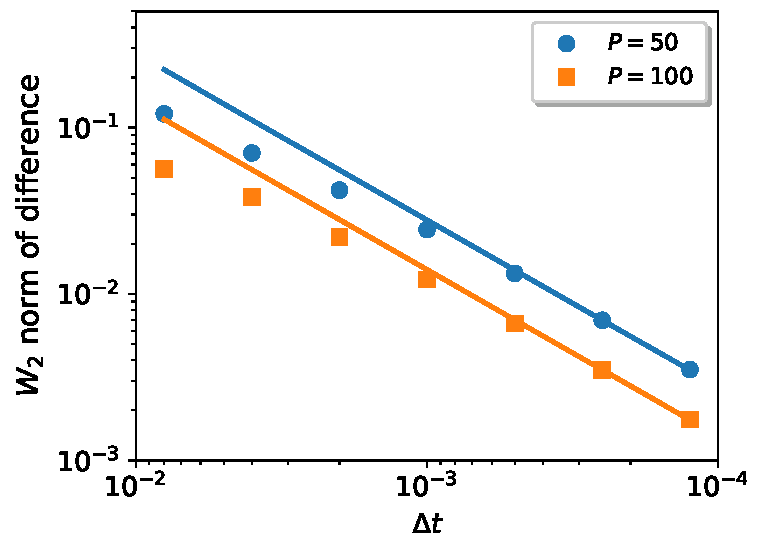
\includegraphics[width=0.6\textwidth]{figs/Energy_3_1.pdf}
\caption{ {The difference on the ensemble average of the total potential energy $\mathscr{P}(U)$ as a function of time step $\Delta t$ (unit: $\tau$). Data are shown for the same systems used in producing Figs.~\ref{fig:3_1} and $P=50$ and $100$. The solid lines indicate $\mathcal{O}(\Delta t)$ scaling. The $W_2$ norm is used as the measurement.}}
\label{fig:energy2d_3_1}
\end{center} 
\end{figure}

\begin{figure}[htb]
\begin{center}
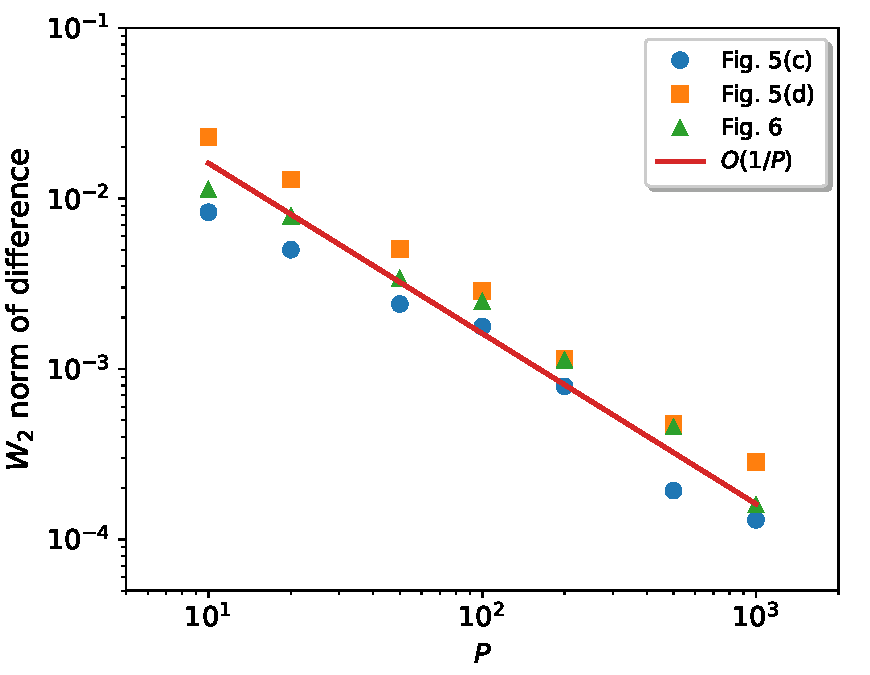
\includegraphics[width=0.6\textwidth]{figs/Energy.pdf}
\caption{The difference on the ensemble average of the total potential energy $\mathscr{P}(U)$ as a function of batch size $P$. Data are shown for the same systems used in producing Figs.~\ref{fig:den1}(c-d) and \ref{fig:den2}. The $W_2$ norm is used as the measurement.}
\label{fig:energy2d}
\end{center} 
\end{figure}

\begin{figure}[!ht]
\begin{center}
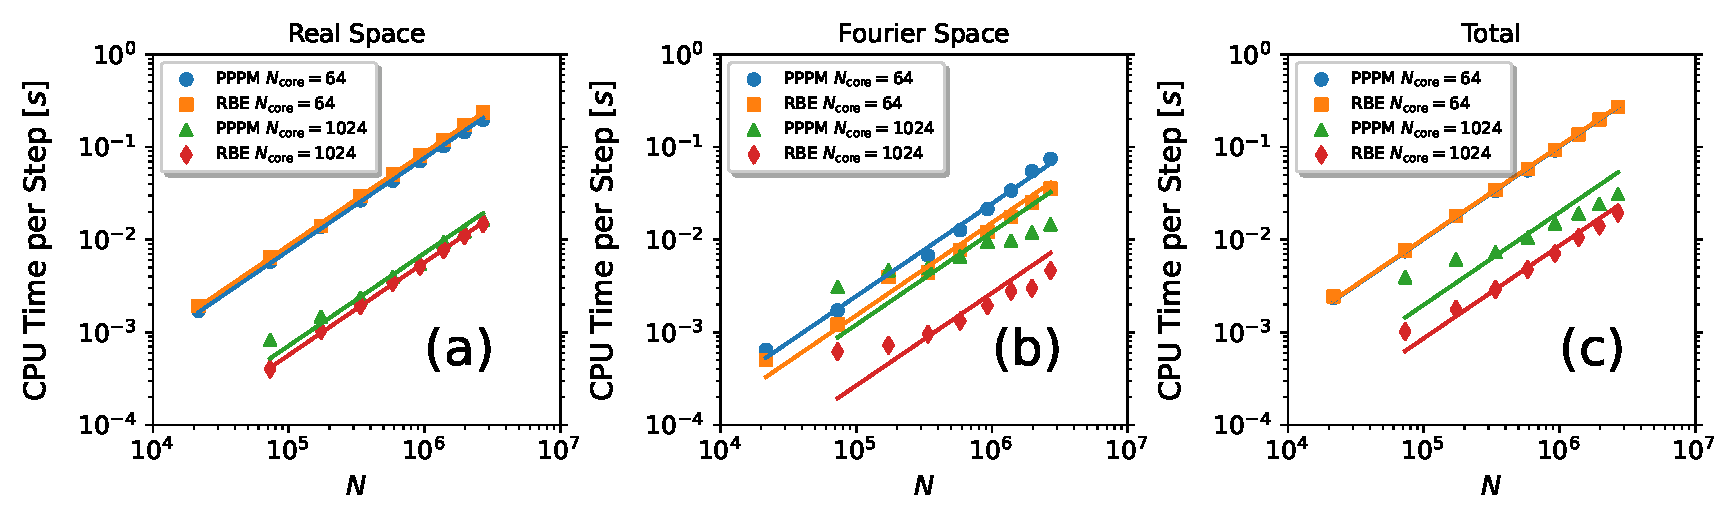
\includegraphics[width=1\textwidth]{figs/time_compare_nonsub.pdf}
\caption{CPU time comparison between the RBE2D and PPPM methods, with the number of CPU cores set to $64$ or $1024$ ($64$ cores per node) and a batch size of $P=200$. Data are shown for the same systems used in producing Fig.~\ref{fig:Time}(a), including CPU time per step of the real space component (Real), the Fourier space component (Fourier), and the total computation time (Total).
The results indicate that while the speedup achieved by the RBE2D method is minimal when the number of CPU cores is small ($N_{\mathrm{core}} = 64$), it becomes significantly more effective at reducing CPU time costs compared to the PPPM method when $N_{\mathrm{core}} = 1024$, primarily due to its lower communication overhead.
Note that in panel (c) the data points marked with blue circles are overlapped by those marked with orange squares.}
\label{fig:timenondie}
\end{center} 
\end{figure}

\begin{figure}[!ht]
\begin{center}
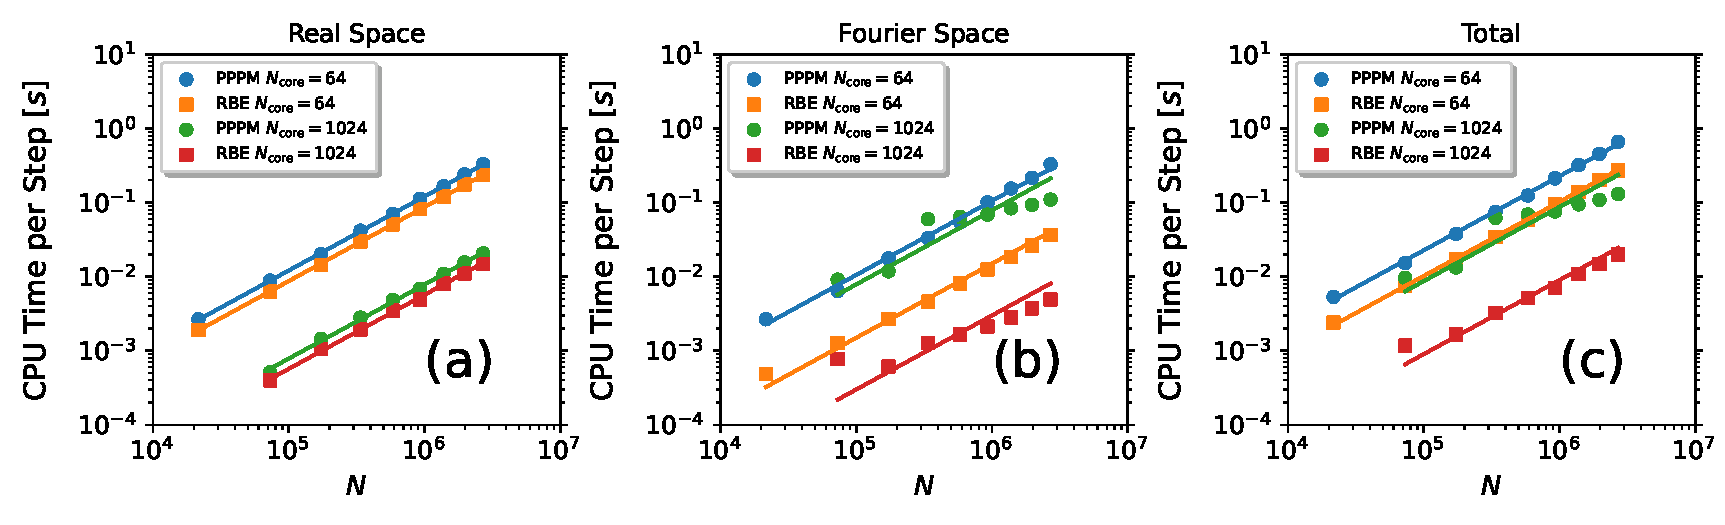
\includegraphics[width=1\textwidth]{figs/time_compare_withsub.pdf}
\caption{ {CPU time comparison between the RBE2D and ICM-PPPM methods, with the number of CPU cores set to $64$ or $1024$ ($64$ cores per node) and a batch size of $P=200$. Data are shown for the same systems as in Fig.~\ref{fig:Time}(a), but with a dielectric mismatch of $\gamma_{\emph{top}} = \gamma_{\emph{bot}} = -0.9$. The CPU time per step is provided for the real space component (Real), Fourier space component (Fourier), and total computation time (Total).
Similarly, the results clearly show the speedup of the RBE2D method over the ICM-PPPM method, especially when the number of CPU cores is large.}}
\label{fig:timedie}
\end{center} 
\end{figure}